\documentclass[12pt,oneside]{uhthesis}
\usepackage{subfigure}
\usepackage[ruled,lined,linesnumbered,titlenumbered,algochapter,spanish,onelanguage]{algorithm2e}
\usepackage{amsmath}
\usepackage{amssymb}
\usepackage{amsbsy}
\usepackage{caption,booktabs}
\captionsetup{ justification = centering }
%\usepackage{mathpazo}
\usepackage{float}
\setlength{\marginparwidth}{2cm}
\usepackage[spanish]{todonotes}
\usepackage{listings}
\usepackage{xcolor}
\usepackage{multicol}
\usepackage{graphicx}
\floatstyle{plaintop}
\restylefloat{table}
\addbibresource{Bibliography.bib}
% \setlength{\parskip}{\baselineskip}%
\renewcommand{\tablename}{Tabla}
\renewcommand{\listalgorithmcfname}{Índice de Algoritmos}
%\dontprintsemicolon
\SetAlgoNoEnd

\definecolor{codegreen}{rgb}{0,0.6,0}
\definecolor{codegray}{rgb}{0.5,0.5,0.5}
\definecolor{codepurple}{rgb}{0.58,0,0.82}
\definecolor{backcolour}{rgb}{0.95,0.95,0.92}

\lstdefinestyle{mystyle}{
    backgroundcolor=\color{backcolour},   
    commentstyle=\color{codegreen},
    keywordstyle=\color{purple},
    numberstyle=\tiny\color{codegray},
    stringstyle=\color{codepurple},
    basicstyle=\ttfamily\footnotesize,
    breakatwhitespace=false,         
    breaklines=true,                 
    captionpos=b,                    
    keepspaces=true,                 
    numbers=left,                    
    numbersep=5pt,                  
    showspaces=false,                
    showstringspaces=false,
    showtabs=false,                  
    tabsize=4
}

\lstset{style=mystyle}

\newenvironment{proof}{\noindent\textbf{Demostraci\'on }}{\hfill $\blacksquare$\\}

\title{Implementaci\'on de un Sistema de Votaci\'on Representativa sobre Quorum}  
\author{\\\vspace{0.25cm}Andy Ledesma Garc\'ia}
\advisor{\\\vspace{0.25cm}Yaidir Mustelier Ruiz}
\degree{Licenciado en Ciencia de la Computación}
\faculty{Facultad de Matemática y Computación}
\date{28 de noviembre de 2022\\\vspace{0.25cm}\href{https://github.com/ic-matcom/rvote-quorum}{https://github.com/ic-matcom/rvote-quorum}}
\logo{Graphics/uhlogo}
\makenomenclature

\renewcommand{\vec}[1]{\boldsymbol{#1}}
\newcommand{\diff}[1]{\ensuremath{\mathrm{d}#1}}
\newcommand{\me}[1]{\mathrm{e}^{#1}}
\newcommand{\pf}{\mathfrak{p}}
\newcommand{\qf}{\mathfrak{q}}
%\newcommand{\kf}{\mathfrak{k}}
\newcommand{\kt}{\mathtt{k}}
\newcommand{\mf}{\mathfrak{m}}
\newcommand{\hf}{\mathfrak{h}}
\newcommand{\fac}{\mathrm{fac}}
\newcommand{\maxx}[1]{\max\left\{ #1 \right\} }
\newcommand{\minn}[1]{\min\left\{ #1 \right\} }
\newcommand{\lldpcf}{1.25}
\newcommand{\nnorm}[1]{\left\lvert #1 \right\rvert }
\renewcommand{\lstlistingname}{Ejemplo de código}
\renewcommand{\lstlistlistingname}{Ejemplos de código}

\begin{document}

\frontmatter
\maketitle

\begin{dedication}
    A mis padres.
\end{dedication}
\begin{acknowledgements}
    Agradezco a mi familia, especialmente a mis padres, por su apoyo incondicional, por cubrir mi retaguardia y, a la vez, estar en la primera l\'inea de combate.

    Muchas gracias a todos mis compa\~neros, por su amistad y ayuda. A Omar, por ser mi hermano y estar codo a codo conmigo en los buenos y malos momentos. A Pablo y Claudia, por acogerme en sus hogares y dejarme ser parte del equipo. A Deborah, por hacerme re\'ir en d\'ias soleados y grises.

    Agradezco a los profesores que trabajan duro para mantener bien en alto el rigor, la calidad y el prestigio de la facultad. Especialmente, al profesor Somoza, por sus magn\'ificas clases y ense\~nanzas.

    Por \'ultimo, pero no menos importante, agradezco a mi tutor, por su gu\'ia y preocupaci\'on.
\end{acknowledgements}
\begin{resumen}
	Resumen en espanyol
\end{resumen}

\begin{abstract}
	Resumen en inglés
\end{abstract}
\tableofcontents
\listoffigures
% \listoftables
\listofalgorithms

\mainmatter

\chapter*{Introducción}\label{chapter:introduction}
\addcontentsline{toc}{chapter}{Introducción}



El Estado cubano pide dinero prestado a entidades de la econom\'ia a trav\'es del Banco Central de Cuba. El monto solicitado y el inter\'es m\'aximo con el que se devolver\'a se plasman en un documento llamado bono soberano.  Los posibles prestamistas participan en una subasta por el bono y el que menor tasa de inter\'es exija por el pr\'estamo ser\'a el ganador, y el Estado pasar\'a a ser su prestatario.  Para decidir qui\'enes participan en la subasta, se confeccionan los Comit\'es de Mercado Financiero (CMF).  Los miembros y el presidente de cada Comit\'e se deciden mediante un proceso electoral en el que cualquier elector puede ceder su poder de voto a otro elector. A ese tipo de elecci\'on el autor le denomina \textbf{votaci\'on representativa}.  


En un sistema de votaci\'on representativa  los votos se transfieren, esto es, si una persona $A$ vota por una persona $B$ y esta, a su vez, vota por  $C$, entonces el voto de $A$ se transfiere a $C$. En el caso particular de la confecci\'on de los CMF, cada individuo puede votar por a lo sumo otra persona.

La figura \ref{fig:r-voting} ilustra un ejemplo de votación en el que $A$ votó por $B$, $B$ y $E$ votaron por $C$ y $C$ votó por $D$. $B$ obtiene solamente el voto de $A$, mientras que $C$ obtiene los votos de $A$, $B$ y $E$. $D$ recibe el voto directo de $C$ y, con este,  los votos indirectos de los restantes participantes.

\begin{figure}[h]
    \centering
    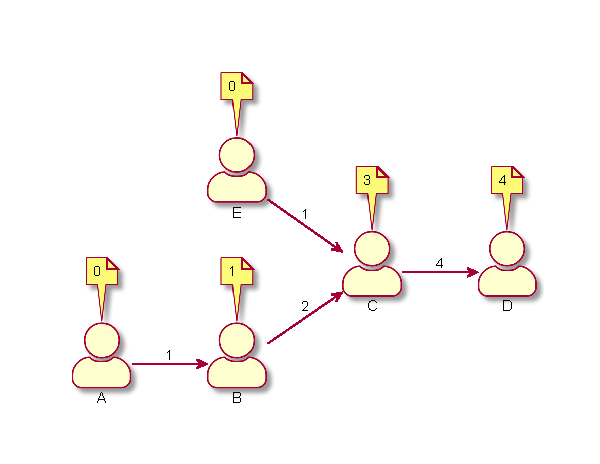
\includegraphics{Graphics/rep-voting.pdf}
    \caption{Conteo de votos en votación representativa.}
    \label{fig:r-voting}
\end{figure}

En un proceso electoral de este tipo pueden surgir ciclos de votación, como el que se muestra en la figura \ref{fig:voting-cycle}, donde el voto emitido por $D$ hacia $B$ forma un ciclo que los involucra a ambos y a $C$. En tal caso, no queda claro cu\'antos votos otorgarle a las personas involucradas en el ciclo.  Uno de los objetivos del presente trabajo es \textbf{dise\~nar e implementar una asignaci\'on justa de  votos para los electores involucrados en un ciclo de votación}. 

\begin{figure}[h]
    \centering
    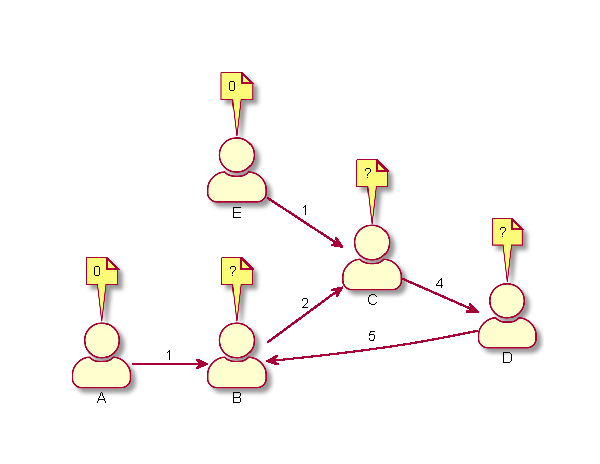
\includegraphics{Graphics/voting-cycle.pdf}
    \caption{Ciclo de votaci\'on.}
    \label{fig:voting-cycle}
\end{figure}

Para seleccionar un presidente para un CMF, se realiza una elecci\'on representativa y el que obtenga la mayor cantidad de votos es el ganador. Puede pasar que m\'as de una persona obtenga la mayor cantidad de votos.   Esto no es deseable, ya que el presidente debe ser \'unico. En este sentido, otro de los objetivos de este trabajo es \textbf{dise\~nar e implementar un mecanismo de desempate}.

% pa mantener un sistema distribuido de goquorum es necesario al menos 4 nodos % @NOTE chekea eso 

Tradicionalmente en estas elecciones, como en muchas otras, los votos son emitidos en boletas de papel y el conteo es realizado manualmente. Esto puede traer consigo ciertos problemas que causan desconfianza en el electorado, como son los votos falsos y el mal conteo de los votos.   Si no se hace una verificaci\'on rigurosa de la identidad del votante, entonces se puede emitir votos con relativa facilidad en nombre de personas que no han votado (votos falsos). Si el conteo no est\'a supervisado adecuadamente, pueden surgir errores en los resultados, ya sea por intereses personales o errores humanos.

En un sistema de votaci\'on electr\'onico se  pueden lograr diversas formas de verificaci\'on biom\'etrica, por ejemplo, mediante la huella digital o el esc\'aner ocular. Por otro lado, en estos sistemas se puede contar los votos de manera eficiente mientras se van realizando y se  puede publicar en vivo los resultados. 

Otras bondades poseen los sistemas electrónicos, como son la flexibilidad, lo fácil que pueden ser de usar y lo baratos que resultan con respecto a los sistemas tradicionales. Sin embargo, muchos de los sistemas electrónicos existentes son centralizados, esto es, dependen de que una agencia central se encargue de registrar, manejar, calcular y revisar los votos. Toda la confianza debe entonces ser depositada en esa agencia, lo cual hace vulnerable al sistema.
 
Un sistema digital descentralizado de votación no tiene ese problema. Una de las tecnologías descentralizadas empleadas actualmente es \textit{blockchain}.   \textit{Blockchain} es un registro distribuido e inmutable  de transacciones. Lo que se transacciona puede ser tangible, como son  una casa o dinero en efectivo, o intangible, como son el derecho de autor de una obra o el voto de un elector por un candidato (\cite{blockchain-ibm}). La inmutabilidad y seguridad de este registro se basan en principios de  criptografía, descentralizaci\'on y mecanismos de consenso (\cite{blockch-security-ibm}). 


% Hacerlo con \textit{blockchain} ta bueno xq resuelve la parte m\'as importante de esos problemas. 

Desde el surgimiento de Ethereum se puede implementar comportamientos complejos mediante contratos inteligentes. Ethereum es una plataforma \textit{blockchain} que establece una red p\'ublica que ejecuta y verifica c\'odigo de manera segura. A dicho c\'odigo o al programa que resulta de ejecutarlo se le conoce como contrato inteligente (\cite{eth-aws}).  

No es deseable que el proceso electoral en el CMF se realice en una red p\'ublica, ya que es un proceso que s\'olo concierne a las partes involucradas. Por otro lado, desplegar un contrato inteligente en Ethereum puede costar miles de d\'olares (\cite{eth-deploy}). Estos dos factores hacen que no sea factible realizar la implementaci\'on de este trabajo sobre la red p\'ublica de Ethereum. 

GoQuorum es una implementaci\'on de Ethereum capaz de crear redes privadas y con mecanismos de autorizaci\'on. En GoQuorum tambi\'en se puede personalizar el costo del despliegue de los contratos inteligentes, incluso, puede hacerse nulo. Por todo lo dicho anteriormente, GoQuorum es una buena opci\'on en la que implementar el sistema de votaci\'on representativa del CMF.


Existen implementaciones de sistemas de votaci\'on en otras \textit{blockchain} (\cite{agora}) y tambi\'en en Ethereum (\cite{ovn} y \cite{borda_count}), pero no se conoce ninguna implementaci\'on de un sistema de voto representativo en GoQuorum.

\todo[inline, disable]{@TODO decir que el Instituto de Criptograf\'ia implement\'o un sistema de votaci\'on en hyperledger fabric pero tampoco nos sirve. ?`C\'omo cito eso?}

En \cite{wang2017review} se proponen los requisitos principales y opcionales que debe cumplir todo sistema de votaci\'on electr\'onico. Entre ellos est\'an:
\begin{itemize}
    \item correctitud: los votos deben ser contados correctamente, esto es, todos los votos v\'alidos deben ser contados y los votos inv\'alidos no deben ser contados.

    \item privacidad: no se conoce la decisi\'on del votante.

    \item prevenci\'on del doble voto: un votante no puede emitir la misma boleta dos veces. También se debe evitar que un tercero pueda clonar una boleta previamente emitida por un votante, para registrarla de nuevo a nombre de ese votante.

    \item elegibilidad: s\'olo los votantes autorizados pueden votar.

    \item robustez: poder lidiar con una cierta cantidad de comportamientos incorrectos por parte de los votantes o con una falla parcial del sistema.

    \item justeza: no se calculan los resultados hasta el fin de la votaci\'on.

\end{itemize}

Con el presente trabajo de diploma  se pretende dise\~nar e implementar un sistema de votaci\'on representativa en GoQuorum que cumpla con los requisitos mencionados anteriormente. El sistema debe ser capaz, adem\'as, de realizar elecciones para un CMF, asignando un valor justo de votos para los electores involucrados en un ciclo de votaci\'on y determinando un ganador, incluso cuando hay empate en el primer lugar. El sistema debe ser lo m\'as gen\'erico posible, de forma tal que sea factible su uso m\'as all\'a del entorno bancario.




% estudiar, disenyar y modelar, implementar y evaluar resultados

% @TODO decir d q' va cada capi'tulo

% @NOTE habla en tiempo presente, 3ra persona del singular, e.g. "el autor ha desarrollado", "el autor ha realizado", etc.

% @TODO usa \citep o el ekivalente cuan2 usas babel cuan2 citas adentro d pare'ntesis. Trae opcio'n pa citas mu'ltiples
\chapter{Estado del Arte}\label{chapter:state-of-the-art}

\section{M\'etodo del Desempate Instant\'aneo}
En los sistemas mayoritarios es necesario que un candidato alcance la mayor\'ia de votos (un determinado porcentaje de los votos) para obtener la victoria. Si esto no sucede, entonces se decide el ganador mediante un \textit{ranking} o en posteriores rondas de votaci\'on.

En los sistemas de \textit{ranking}, los electores deben otorgarle un puesto a cada candidato (primero, segundo, tercero, etc.).  Para determinar el ganador, se utilizan m\'etodos como el \textit{desempate instant\'aneo} (IRV, por ``instant-runoff voting'' en ingl\'es). 

En IRV se cuentan los votos de la primera elecci\'on de cada votante. Si un candidato posee m\'as de la mitad de  los votos, entonces gana la elecci\'on. En otro caso, se elimina al candidato con menos votos y se le aumenta un voto a la siguiente opci\'on disponible de todos aquellos que hayan elegido al candidato eliminado en primera opci\'on. Esto \'ultimo puede ser visto como que en toda boleta donde el $i$-\'esimo candidato sea el eliminado, el \textit{ranking} se desplaza, esto es, el $(i+1)$-\'esimo pasa a ser el $i$-\'esimo, el $(i+2)$-\'esimo pasa a ser el $(i+1)$-\'esimo, etc\'etera. El proceso contin\'ua hasta que alg\'un candidato obtenga m\'as de la mitad de los votos. 

La figura \ref{fig:irv} muestra el diagrama de flujo del IRV.

\begin{figure}[!h]
    \centering
    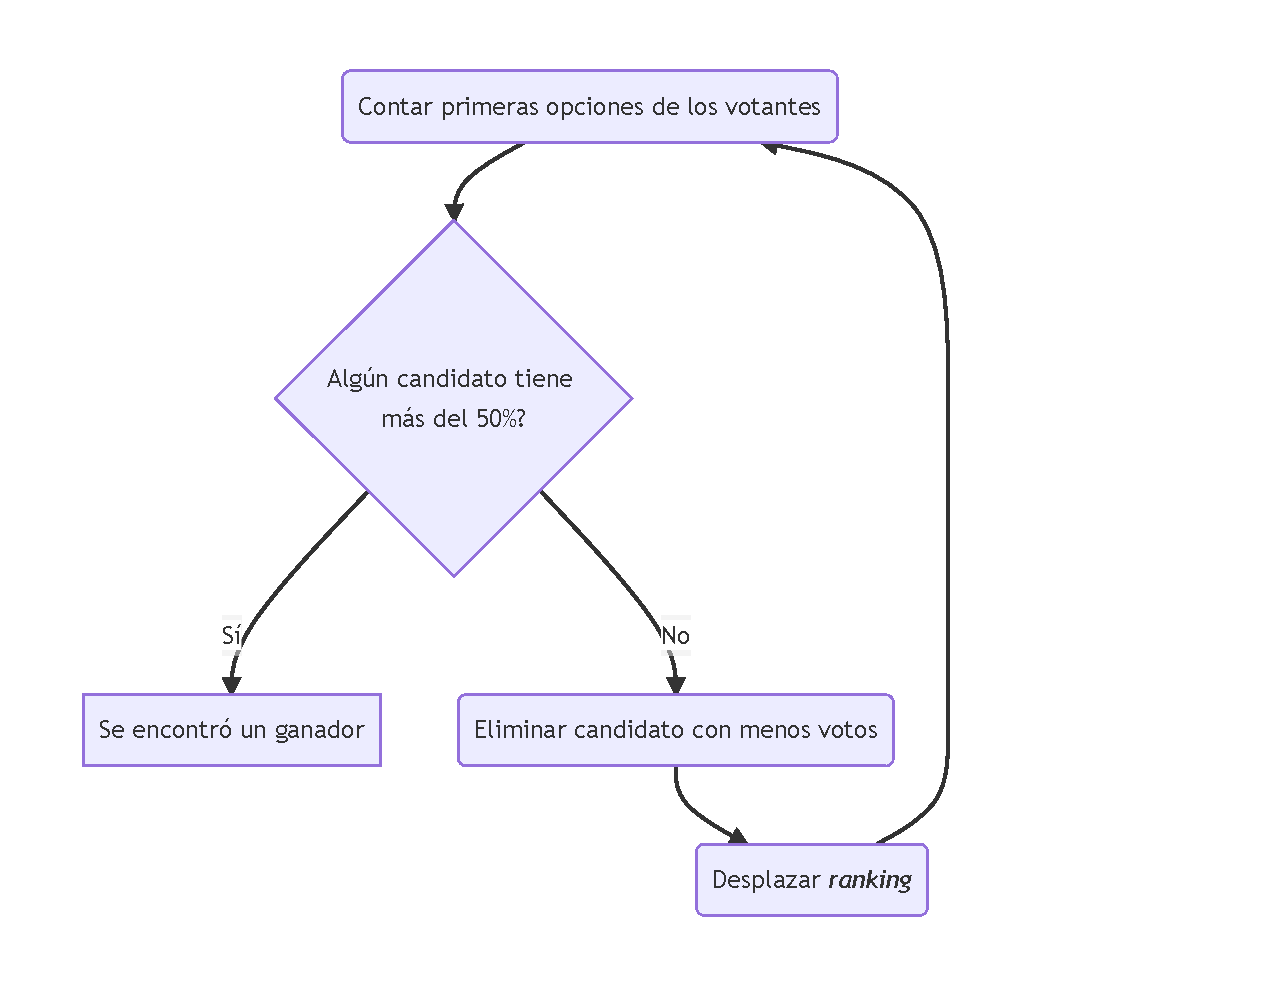
\includegraphics[width=0.8\textwidth]{Graphics/irv.pdf}
    \caption{Diagrama de flujo del m\'etodo de desempate instant\'aneo.}
    \label{fig:irv}
\end{figure}
\chapter{Propuesta}\label{chapter:proposal}

\newcommand{\dfscaption}{\hyperref[algo:dfs]{DFS-Votos}}
\newcommand{\cyclevotescaption}{\hyperref[algo:votes-cycles]{Reasignar-Votos-en-Todos-los-Ciclos}}
\newcommand{\dfsvisitcaption}{\hyperref[algo:dfs-visit]{DFS-Votos-Visita}}
\newcommand{\initdfsvertices}{\hyperref[algo:init-dfs-vertices]{Inicializar-Propiedades-de-V\'ertices}}
\newcommand{\maxincyclecaption}{\hyperref[algo:max-in-cycle]{M\'ax-Votos-en-Ciclo}}
\newcommand{\setvotestoallincyclecaption}{\hyperref[algo:set-votes-all-in-cycle]{Reasignar-Votos-en-Ciclo}}

\section{Conteo de Votos}
Sean $V$ el conjunto de los participantes  de la elecci\'on (votantes) y $f \in V \times V$ la relaci\'on de voto, esto es, $ \langle x, y \rangle \in f $ si y s\'olo si $x$ vot\'o por $ y $.  Se asume que culmin\'o el registro de todos los votos y que s\'olo existen votos v\'alidos. Cada votante puede elegir a lo sumo a otra persona, por ende, $f$ es funci\'on.

Sea $G' = \langle V, f \rangle$ el digrafo de votaci\'on. Representaciones de este grafo pueden ser encontradas en las figuras \ref{fig:r-voting} y \ref{fig:voting-cycle}.

Ahora bien, sea $G = \langle V, f^{-1} \rangle$. Se denota por $G_\pi$ al subgrafo de predecesores del DFS \citep{intro-to-algo-3}. El conteo de los votos obtenidos por $x$ se reduce a contar la cantidad de nodos en el sub\'arbol de $x$ en $G_\pi$. \todo{@TODO demostrarlo}

El conteo de los votos puede ser implementado mediante DFS. En este sentido, los algoritmos \ref{algo:dfs} y \ref{algo:dfs-visit} constituyen adaptaciones   a las propuestas de DFS y DFS-Visit de \cite{intro-to-algo-3}, respectivamente. Se asume que $G$ se encuentra representado mediante listas de adyacencia. En $B$ se almacenan los arcos de retroceso de $G$, los cuales ser\'an empleados posteriormente para asignar los votos a los v\'ertices que se encuentran en alg\'un ciclo.  Una vez el algoritmo \ref{algo:dfs} termine, en $u.votos$ se tendr\'a la cantidad de votos obtenidos por el votante representado mediante el v\'ertice $u$.

\begin{algorithm}[!h]
    \caption{\dfscaption}
    \label{algo:dfs}
    \DontPrintSemicolon
    \SetAlgoLined
    \Entrada{Grafo $G = \langle V, f^{-1} \rangle$.}
    \BlankLine

    \initdfsvertices($G.V$)\;
    $B = \{\}$\;
    \ForEach{v\'ertice $u \in G.V$}{
        \If{$u.color == $ {\rm BLANCO}}{
            \dfsvisitcaption($G, u, B$)\;
        }
    }
    \cyclevotescaption($G, B$)\; \label{algo:dfs:line:votes-in-cycles}
\end{algorithm}

\begin{algorithm}[!h]
    \caption{\initdfsvertices}
    \label{algo:init-dfs-vertices}
    \DontPrintSemicolon
    \SetAlgoLined
    \Entrada{Conjunto de v\'ertices $V$.}
    \BlankLine

    \ForEach{v\'ertice $u \in V$}{
        $u.color =$ BLANCO\;
        $u.candidato =$ NIL\;
        $u.votos = 0$\;
    }
\end{algorithm}

El algoritmo \ref{algo:dfs} difiere en muy pocos aspectos al de \cite{intro-to-algo-3}. Uno de los m\'as significativos es el llamado a la funci\'on Set-Votes-In-Cycles en la l\'inea \ref{algo:dfs:line:votes-in-cycles}. Esta funci\'on se encarga de asignar los votos a los v\'ertices que se encuentran en alg\'un ciclo.  

El algoritmo \ref{algo:dfs-visit} calcula los votos obtenidos por $u$ y a\~nade a $B$ los arcos de retroceso encontrados durante el proceso.

\begin{algorithm}[!h]
    \caption{\dfsvisitcaption}
    \label{algo:dfs-visit}
    \DontPrintSemicolon
    \SetAlgoLined
    \Entrada{Grafo $G$; v\'ertice $u$; conjunto $B$ de arcos de retroceso.}     
    \BlankLine

    $u.color =$ GRIS\;

    \ForEach{$v \in G.Adj[u]$}{ \label{algo:dfs-visit:line:arc-foreach}
        $v.candidato = u$\;
        \If{$v.color ==$ {\rm BLANCO}}{
            \dfsvisitcaption($G, v, B$)\;
        }\lElse{\If{$v.color ==$ {\rm GRIS}}{
            $B = B \cup \{\langle u, v \rangle\}$\; \label{algo:dfs-visit:line:add-B}
        }}
        \If{$v.color ==$ {\rm NEGRO}}{ \label{algo:dfs-visit:line:if-black}
            $u.votos = u.votos + v.votos + 1$\; \label{algo:dfs-visit:line:votes}
        }
    }
    $u.color =$ NEGRO\;
\end{algorithm}

El \textbf{foreach} de las l\'ineas \ref{algo:dfs-visit:line:arc-foreach}-\ref{algo:dfs-visit:line:votes} itera por todos los arcos salientes de $u$. N\'otese que $v \in G.Adj[u]$ si y s\'olo si $v$ vot\'o por $u$, por definici\'on de $G$.  Se a\~nade un nuevo arco de retroceso a $B$ en la l\'inea \ref{algo:dfs-visit:line:add-B}. Un arco $\langle u, v \rangle$ es de retroceso si y s\'olo si $v$ es gris cuando se explora ese arco por primera vez \citep{intro-to-algo-3}. El n\'umero de votos obtenidos por $u$ es actualizado solamente en la l\'inea \ref{algo:dfs-visit:line:votes}, cuando $v$ es negro. Esto se debe a que los votos obtenidos por $v$ se encuentran bien calculados cuando es negro. Todos los votos obtenidos por $v$, m\'as el voto que este le confiere a $u$, son contados como votos de  $u$. N\'otese que el bloque de las l\'ineas \ref{algo:dfs-visit:line:if-black}-\ref{algo:dfs-visit:line:votes} es un \textbf{if}, y no un \textbf{else if}. Esto es intencional y permite que se actualicen los votos de $u$ correctamente, incluso cuando $\langle u, v \rangle$ es un arco de \'arbol de $G_\pi$.

\todo[inline]{@TODO probar q cuan2 v es negro entonces los votos d v esta'n bien contados}

El algoritmo \ref{algo:votes-cycles} itera por todos los ciclos de $G$. En cada ciclo, calcula el mayor n\'umero de votos obtenidos por un v\'ertice del ciclo y le asigna esa cantidad a los restantes v\'ertices del ciclo. Los votantes de un mismo ciclo conf\'ian indirectamente entre ellos dos a dos, por ende, se considera justo que cada uno de ellos obtenga la misma cantidad de votos, y que esta sea la mayor obtenida por un miembro del ciclo.

\begin{algorithm}[!h]
    \caption{\cyclevotescaption}
    \label{algo:votes-cycles}
    \DontPrintSemicolon
    \SetAlgoLined
    \Entrada{Grafo $G$; conjunto $B$ de arcos de retroceso.}     
    \BlankLine

    \ForEach{$\langle u, v \rangle \in B$}{
        $m = $ \maxincyclecaption($\langle u, v \rangle$)\;
        \setvotestoallincyclecaption($m, \langle u, v \rangle$)\;
    }
\end{algorithm}

\todo[inline]{@TODO hay q probar q c esta'n considerando todos los ciclos}

\begin{algorithm}[!h]
    \caption{\maxincyclecaption}
    \label{algo:max-in-cycle}
    \DontPrintSemicolon
    \SetAlgoLined
    \Entrada{Arco de retroceso $\langle u, v \rangle$.}     
    \Salida{Mayor n\'umero de votos obtenidos por un v\'ertice del ciclo.}
    \BlankLine

    $m = v.votos$\;
    $x = u$\;
    \While{$x \neq v$}{
        $m = \max(m, x.votos)$\;
        $x = x.candidato$\;
    }
    \Return{$m$}\;
\end{algorithm}

\todo[inline]{@TODO probar q el ciclo de los algoritmos \ref{algo:set-votes-all-in-cycle} y \ref{algo:max-in-cycle} termina}

\begin{algorithm}[!h]
    \caption{\setvotestoallincyclecaption}
    \label{algo:set-votes-all-in-cycle}
    \DontPrintSemicolon
    \SetAlgoLined
    \Entrada{$m$ votos a asignar; arco de retroceso $\langle u, v \rangle$.}     
    \BlankLine

    $x = u$\;
    \While{$x \neq v$}{
        $x.votos = m$\;
        $x = x.candidato$\;
    }
    $v.votos = m$\;
\end{algorithm}



\section{Implementaci\'on del Desempate}
Sean $m = \max\{ u.votos \;|\; u \in V \}$ y $W = \{ u \in V \;|\; u.votos = m \}$.  Para determinar un ganador cuando $|W| > 1$, se emplea una adaptaci\'on del m\'etodo de desempate instant\'aneo. 

Sea $x \in V$ un v\'ertice cualquiera de $G'$. Sea $P(x)$ un camino simple maximal de $G'$ que comienza en $x$. Luego,
$$
P(x) = \langle x, f(x), f(f(x)), \ldots, f^{k}(x) \rangle.
$$
Como $f$ es funci\'on, entonces $P(x)$ es \'unico. 

Sea $D$ el conjunto de los votantes que han sido eliminados por el m\'etodo de desempate. El \textit{ranking} de $x$ se define como  la subsecuencia maximal de $P(x)$ de v\'ertices que est\'an en $W$ y que no est\'an en $D \cup \{ x \}$. 
% Formalmente, el \textit{ranking} de $x$ es
% $$
% R(x) = \langle y_{i_1}, y_{i_2}, \ldots, y_{i_t} \rangle, \quad 1 \leq i_1 \leq i_2 \leq \ldots \leq i_t \leq k, \quad y_{i_j} \in W \setminus D, \; 1 \leq \forall j \leq t.
% $$
Sea $x \in V$ un v\'ertice cualquiera de $G'$. Sea $P(x)$ un camino simple maximal de $G'$ que comienza en $x$. Luego,
$$
P(x) = \langle x, f(x), f(f(x)), \ldots, f^{k}(x) \rangle.
$$
Como $f$ es funci\'on, entonces $P(x)$ es \'unico. 

Sea $D$ el conjunto de los votantes que han sido eliminados por el m\'etodo de desempate. El \textit{ranking} de $x$ se define como  la subsecuencia maximal de $P(x)$ de v\'ertices que est\'an en $W$ y que no est\'an en $D \cup \{ x \}$. 
% Formalmente, el \textit{ranking} de $x$ es
% $$
% R(x) = \langle y_{i_1}, y_{i_2}, \ldots, y_{i_t} \rangle, \quad 1 \leq i_1 \leq i_2 \leq \ldots \leq i_t \leq k, \quad y_{i_j} \in W \setminus D, \; 1 \leq \forall j \leq t.
% $$
\chapter{Detalles de Implementación y Experimentos}\label{chapter:implementation}


\backmatter

\begin{conclusions}
    \todo[inline]{@audit debes responder la pregunta objetiva de la tesis}

    En este trabajo se model\'o el problema desde la Teor\'ia de Grafos y  se contaron los votos obtenidos por cada candidato mediante una B\'usqueda del Primero en Profundidad. A los candidatos involucrados en ciclos de votaci\'on se les reasignaron los votos siguiendo un criterio justo. El algoritmo se ejecuta en tiempo lineal con respecto al n\'umero de participantes.

    Se emple\'o el M\'etodo de Desempate Instant\'aneo (IRV) para escoger un ganador cuando existe empate en el primer lugar. Este m\'etodo de desempate no necesita de una segunda ronda de elecciones y es totalmente autom\'atico. El algoritmo se ejecuta en tiempo $O(n \log n)$, donde $n$ es el total de participantes.
    
    Se tuvo en cuenta el tiempo de los votos a la hora de eliminar un candidato  en cada iteraci\'on del IRV. Se demostr\'o que es \'unico el candidato a eliminar siempre que se garantice que dos votantes no voten al mismo tiempo. Si bien es un criterio sencillo de implementar, no es quiz\'as el m\'as adecuado cuando los votantes conocen con tiempo suficiente qui\'enes son los candidatos. Esto se debe a que en esas circunstancias se est\'a premiando a un candidato sobre otro por algo que tiene poco que ver con su propuesta electoral. Por otro lado, el criterio incentiva a registrar el voto lo m\'as r\'apido posible, lo cual contribuye a que  el proceso electoral culmine en poco tiempo.

    Se implement\'o un contrato inteligente en  Solidity que ofrece funcionalidades b\'asicas para la realizaci\'on de elecciones representativas. El creador del contrato (due\~no) registra a los votantes autorizados y tiene acceso a funcionalidades administrativas. El due\~no tiene demasiado poder: s\'olo es necesaria su aprobaci\'on para registrar a los votantes, puede registrar votos de terceros e inhabilitar el contrato. Por otro lado, cualquier usuario puede conocer qui\'en va ganando las elecciones en cualquier momento. Esto puede considerarse injusto en muchos entornos, ya que puede predisponer la decisi\'on del votante.

    Implementar el contrato en Solidity permite que pueda ser desplegado en cualquier cliente de Ethereum. GoQuorum es uno de esos clientes que permite la realizaci\'on de transacciones privadas, las cuales pueden ser empleadas para ocultar las decisiones de los votantes. \todo{@audit va en el capt 3}
    
    El contrato fue evaluado en una red privada de GoQuorum, obteni\'endose resultados satisfactorios.
\end{conclusions}

\begin{recomendations}
    Se recomienda analizar con detenimiento la complejidad temporal del algoritmo de desempate, ya que puede que en casos con pocos participantes sea m\'as eficiente emplear un algoritmo $\Theta(n^2)$. 
    
    Se debe considerar el empleo de un criterio de eliminaci\'on de votantes para IRV que se adapte mejor a los entornos donde los votantes conocen con tiempo suficiente qui\'enes son los candidatos.

    El contrato debe ser redise\~nado para restarle poder al due\~no cuando as\'i se desee. Por ejemplo, se puede obligar a que la creaci\'on del contrato  necesite la firma de varias personas. Por otro lado, en  entornos donde se necesite un sistema electoral justo, se debe eliminar la posibilidad de conocer qui\'en va ganando las elecciones en cualquier momento. 
\end{recomendations}

\begin{opinion}
    Opiniones de los tutores
\end{opinion}
\printbibliography[heading=bibintoc]

\end{document}